\chapter{Метод гибкого сравнения на графах}

Метод гибкого сравнения на графах -- метод обработки изображений и распознавания образов, который 
используется для нахождения соответствия между двумя изображениями, учитывая возможные искажения, изменение масштаба и повороты~\cite{distances}.

Данный метод является одним из способов распознования лиц.
Лица представлены в виде графов со взвешенными
вершинами и ребрами\cite{wen}. 
Во время распознавания один из графов –- константный(эталонный), 
в то время как другой изменяется(деформируется) с 
целью наилучшей подгонки к первому. 

В данном методе графы могут представлять собой как 
прямоугольную решетку (рис. \ref{img:ant}.a), так и структуру, образованную антропометрическими
точками лица(рис. \ref{img:ant}.б).

\begin{figure}[h]
    \centering
    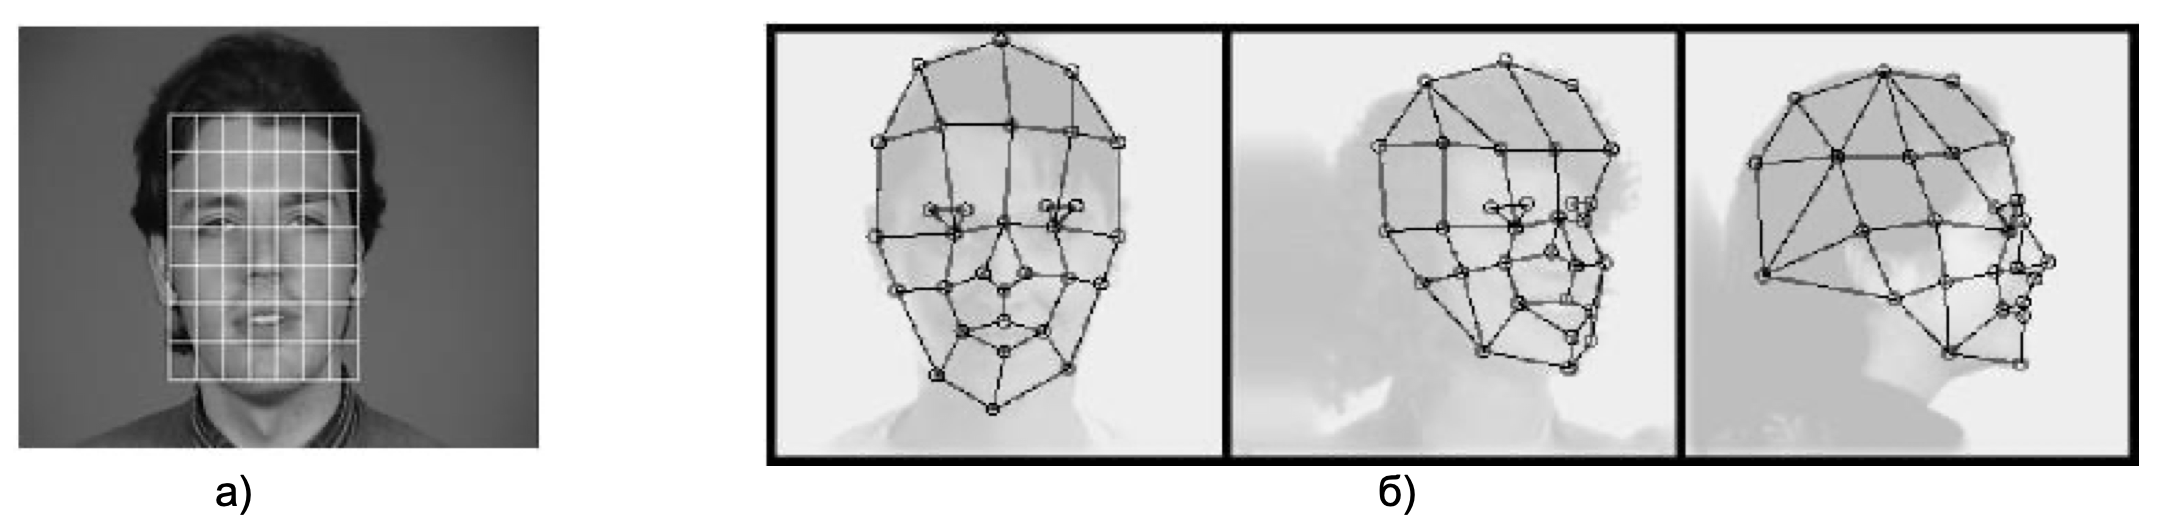
\includegraphics[height=0.15\textheight]{img/ex.jpg}
    \caption{Примеры структуры графа для распознования лиц: \\ 
    a)регулярная решетка; \\ б)граф на основе антропометрических точек лица.}
    \label{img:ant}
\end{figure}

Частотное содержимое изображения --- характеристика, показывающая насколько быстро 
меняется яркость или цвет в различных частях изображения~\cite{chst}.

Фильтр Габора --- фильтр, который анализирует, присутствует ли какое-либо конкретное частотное содержимое 
в изображении в различных направлениях в области вокруг точки или области анализа. Данный фильтр представляет собой 
синусоидальную плоскую волну(рис. \ref{img:sinuso}).\cite{gb}
\begin{figure}[h]
    \centering
    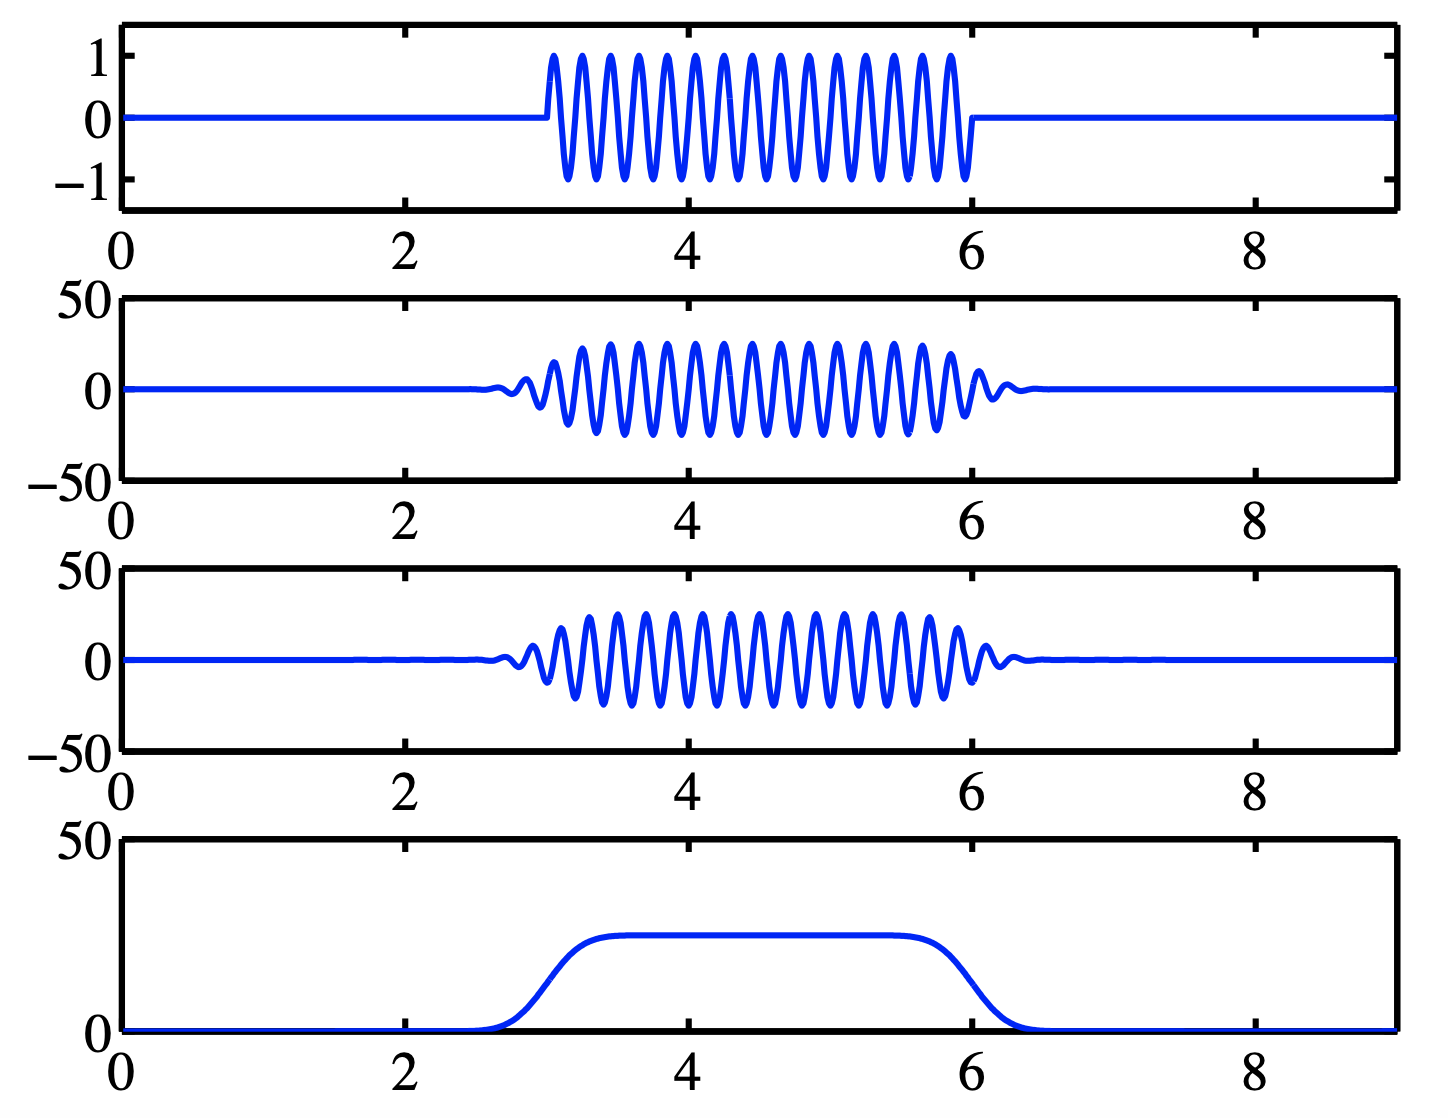
\includegraphics[width=0.35\textheight]{img/sin.png}
    \caption{Пример синусоидальной плоской волны.}
    \label{img:sinuso}
\end{figure}

\vspace{\baselineskip}
\vspace{\baselineskip}
\vspace{\baselineskip}
\vspace{\baselineskip}
\vspace{\baselineskip}
\vspace{\baselineskip}
\vspace{\baselineskip}

Свертка -- операция вычисления нового значения интенсивности, степени яркости
светлых пикселей по сравнению с более темными тонами,
заданного пикселя, при котором учитываются значения окружающих его соседних пикселей.

В некоторой локальной области вершины графа вычисляют значения
путем свертки значений яркости пикселей с набором фильтров Габора(рис. \ref{img:gabnab} -- \ref{img:gab}).

\begin{figure}[h]
    \centering
    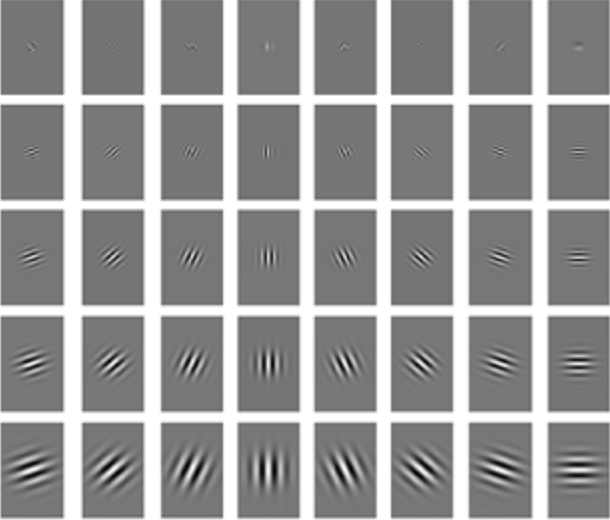
\includegraphics[height=0.35\textheight]{img/img_b.jpg}
    \caption{Набор фильтров Габора.}
    \label{img:gabnab}
\end{figure}
\vspace{\baselineskip}
\vspace{\baselineskip}
\vspace{\baselineskip}
\vspace{\baselineskip}
\vspace{\baselineskip}

\begin{figure}[h]
    \centering
    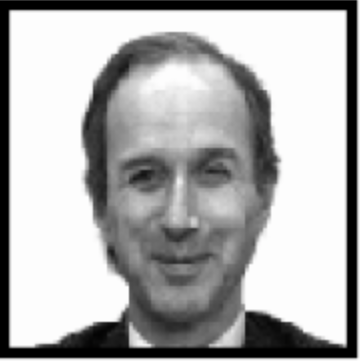
\includegraphics[height=0.15\textheight]{img/gbr1.png}
    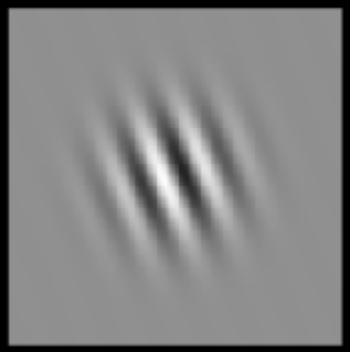
\includegraphics[height=0.15\textheight]{img/gbr2.png}
    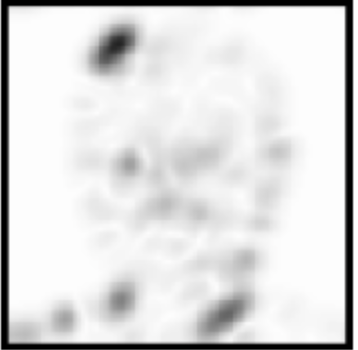
\includegraphics[height=0.15\textheight]{img/gbr3.png}
    \caption{Пример свертки изображения лица с фильтрами Габора.}
    \label{img:gab}
\end{figure}

\textbf{Алгоритм распознования лица:}
\begin{enumerate}
    \item Происходит деформация графа путем смещения каждой из его вершин на некоторое расстояние
    в различных направлениях относительно его исходного местоположения(рис. \ref{img:demonstration});
    \item Выбирается такая позиция, при которой разница между значениями в вершине деформируемого графа и 
    соответствующей ей вершине эталонного графа будет минимальной;
    \item Данная операция выполняется поочердено для всех вершин графа, пока не будет достигнуто наименьшее суммарное различие 
    между признаками этих графов;
    \item  Данная процедура деформации выполняется для всех эталонных лиц, заложенных в базу данных системы. 
    Результат распознавания -- эталон с наименьшим суммарным различием.
\end{enumerate}

\begin{figure}[h]
    \centering
    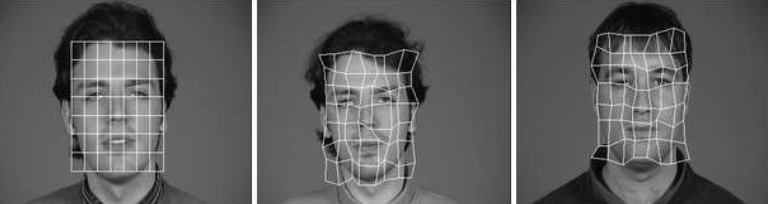
\includegraphics[height=0.15\textheight]{img/img_a.jpg}
    \caption{Пример деформации графа.}
    \label{img:demonstration}
\end{figure}
    
